%%%%%%%%%%%%%%%%%%%%%%%%%%%%%%%%%%%%%%%%%%%%%%%%%%%%%%%%%%%%%%%%%%%%%%%%%%%%
% AGUJournalTemplate.tex: this template file is for articles formatted with LaTeX
%
%%%%%%%%%%%%%%%%%%%%%%%%%%%%%%%%%%%%%%%%%%%%%%%%%%%%%%%%%%%%%%%%%%%%%%%%%%%%

%% To submit your paper:
\documentclass[draft]{agujournal2019}
\usepackage{url}
\usepackage{lineno}
\usepackage[inline]{trackchanges}
\usepackage{soul}
\linenumbers

\draftfalse

\journalname{Geophysical Research Letters}

\begin{document}

%%%%%%%%%%%%%%%%%%%%%%%%%%%%%%%%%%%%%%%%%%%%%%%
%  TITLE
%%%%%%%%%%%%%%%%%%%%%%%%%%%%%%%%%%%%%%%%%%%%%%%

\title{Record low runoff efficiency in the Upper Coloardo during water year 2026} 
% DRAFT working title -- revisit once the analysis is finalized.

%%%%%%%%%%%%%%%%%%%%%%%%%%%%%%%%%%%%%%%%%%%%%%%
%  AUTHORS AND AFFILIATIONS
%%%%%%%%%%%%%%%%%%%%%%%%%%%%%%%%%%%%%%%%%%%%%%%

\authors{=list all authors here=}

\affiliation{1}{=Affiliation Address=}

\correspondingauthor{=name=}{=email address=}

%%%%%%%%%%%%%%%%%%%%%%%%%%%%%%%%%%%%%%%%%%%%%%%
% KEY POINTS
%%%%%%%%%%%%%%%%%%%%%%%%%%%%%%%%%%%%%%%%%%%%%%%
% DRAFT -- each must stay under 140 characters, no special punctuation, complete sentences.

\begin{keypoints}
\item
\end{keypoints}

%%%%%%%%%%%%%%%%%%%%%%%%%%%%%%%%%%%%%%%%%%%%%%%
%  ABSTRACT and PLAIN LANGUAGE SUMMARY
%%%%%%%%%%%%%%%%%%%%%%%%%%%%%%%%%%%%%%%%%%%%%%%

\begin{abstract}

\end{abstract}

\section*{Plain Language Summary}

%%%%%%%%%%%%%%%%%%%%%%%%%%%%%%%%%%%%%%%%%%%%%%%
%
%  BODY TEXT -- OUTLINE ONLY
%
%  Per instruction: sections + talking points, not full prose. Bulleted
%  outline notes below are working notes for drafting, not AGU-style final
%  text (AGU discourages bullets in the published version -- convert each
%  bullet to prose before submission).
%
%%%%%%%%%%%%%%%%%%%%%%%%%%%%%%%%%%%%%%%%%%%%%%%

\section{Background}
\begin{itemize}
\item Colorado river flow (``runoff") is very important for the western USA.
\item Mass balance dictates, Runoff = Precipitation  - Evaporation +/- change in storage.
\item We normally can assume +/- change in storage is small. 
\item The year to year variation in precipitation drives a substantial amount of the variability in runoff.
\item Emerging evidence suggests an \textit{increasing sensitivity of runoff to air temperature} (e.g., \citeA{Woodhouse2016-tb}).
\item Temperature is related to the Evaporation term in a number of direct and indirect ways, likely mediated through snow \cite{Milly2018-yo, Milly2020-nk}.
\item Annual runoff anomalies are commonly modelled as $\Delta Q = \alpha \Delta P + \beta \Delta T$ where $\Delta X = \frac{X-\hat{X}}{\bar{X}}$ for precipitation and runoff, and $\Delta T= T - \bar{T}$ \cite{Lehner2017-se, Milly2020-nk}. The ``bar'' symbol denotes the long term mean.
\item Thus, we can estimate $\alpha$ and $\beta$ based on observed data of precipitation, temperature, and runoff. 
\item For this work, I would also like to include peak springtime SWE as another predictor —-- which may exercise an independent effect on runoff but is itself highly correlated with P and T. 
\item \textbf{2026 was incredibly anomalous} -- it was the warmest year on record, runoff was the third lowest ever measured, springtime snow storage was the lowest on record \cite{Marshall2026-sy}, and most critically — precipitation was low but not extrordinarily low.

\end{itemize}


\section{Goals/questions}

\begin{itemize}
\item How anomalous was 2026?
\item Did 2026 ``break' models of runoff sensitivity to temperature, precipitation, and SWE? Or do pre-2026 estimates of $\alpha$ and $\beta$ still well describe runoff in 2026?
\item SWE was very low, but precipitation was not as unusual. Does the data support the hypothesis that the SWE anomaly had a clear effect (independent of P and T) on the runoff ratio in 2026?
\item Based on these insights, how much more likely is WY2026 runoff by the end of century? (e.g., it's a 1 in 20 year event, by 2080 it's 1 in 5).  
\end{itemize}



\section{Results (highly preliminary)}
\subsection{Historical context of 2026}
\begin{itemize}
    \item Fig \ref{fig:historical} shows the historical trends, since 1906, of temperature, precipitation, runoff, and runoff ratio. 
    \item 2026 was the warmest on record (z=4.3), had the lowest runoff ratio, the third lowest streamflow, and the lowest peak SWE ever observed. 
    \item We can apply the estimate the coefficients for the equation $Q' = \alpha P' + \beta T'$ based on the data in Fig. \ref{fig:historical}
    \item Table 1 shows the coefficients $\alpha$ and $\beta$ fit to data from 1936. These is basically identical to the coefficients in \citeA{Lehner2019-hs}, Fig. 3. 
    \item An $\alpha$ of 1.37 means that a 1$\%$ increase in precipitation yields a $1.37$ percent increase in runoff. 
    \item A $\beta$ of -10.9 means that a 1$^\circ$ degree increase in annual air temperature reduces runoff by 10.9$\%$.
    \item Including the effect of SWE reduces the temperature and precipitation sensitivity substantially — $\alpha$ goes from 1.29 to 1.05 and $\beta$ is also reduced. 
    \item Including SWE also improves the $R^2$.
    \item $\beta$ has a large confidence range, which seems bad. 
\end{itemize}



\begin{table}[h]
\caption{Regression coefficients ($\pm$ 95\% confidence interval) for runoff and spring SWE anomalies, WY1936--2026 ($n= 90$). 
$R^2$ is uncentered.
}
\centering
\begin{tabular}{l l c c c c c}
\hline
Response & Predictors & Eq. & $\alpha_{tot}$ & $\beta_{tot}$  & $\gamma$  & $R^2$ \\
\hline
$\Delta Q$ & $\Delta P, \Delta T$ & \ref{eq:q_model} & $1.29 \pm 0.20$ & $-10.0 \pm 4.2$ & -- & 0.75 \\
$\Delta SWE$ & $\Delta P, \Delta T$ & \ref{eq:swe_model} & $0.53 \pm 0.25$ & $-12.9 \pm 5.1$ & -- & 0.44 \\
$\Delta Q$ & $\Delta P, \Delta T, \Delta SWE$ & \ref{eq:q_total} & $1.05 \pm 0.19$ & $-4.1 \pm 4.0$ & $0.45 \pm 0.14$ & 0.83 \\
\hline
\end{tabular}
\label{tab:coefs}
\end{table}

\subsection{Looking forward}
\begin{itemize}
    \item I am simply taking the coefficients $\alpha$ and $\beta$ and using those to estimate $Q$ anomalies based on projections of T and P from WUS-D3. 
    \item I am not using WUS-D3's own "runoff" variable — rather just precipitation, temperature, and springtime SWE from the models. 
\end{itemize}

\begin{itemize}
    \item Runoff and runoff ratio are projected to decline. 
    \item Including SWE reduces the rate of runoff decline versus P and T only. 
    \item This is likely because of non-linearities between annual warming abd annual precipitation and spring SWE.
    \item 
\end{itemize}

%%%%%%%%%%%%%%%%%%%%%%%%%%%%%%%%%%%%%%%%%%%%%%%
% REFERENCES and BIBLIOGRAPHY
%%%%%%%%%%%%%%%%%%%%%%%%%%%%%%%%%%%%%%%%%%%%%%%



% Following \citeA{Lehner2017-se} and other works, we start by defining runoff sensitivities to temperature and precipitation 

% we define $x' = \mathrm{ln} x - \mathrm{ln} \bar{x}$. and $\mathrm{ln}(x')$ for temperature.
% The Runoff Ratio (RR) is given by $\frac{Q}{P}$. 
% Therefore, in log-space, $RR' = \Delta Q - \Delta P$.

% We can then express the sensitivity to precipitation, temperature, and snow water equivalent using the following expression where $\alpha$, $\beta$, and $\epsilon$ are elasticities.

% \begin{equation}
% \Delta RR = (1 - \alpha) \Delta P + \beta \Delta T + \gamma \Delta SWE + \epsilon
% \end{equation}

% We can make a linear model of model SWE as the 



\begin{figure}
    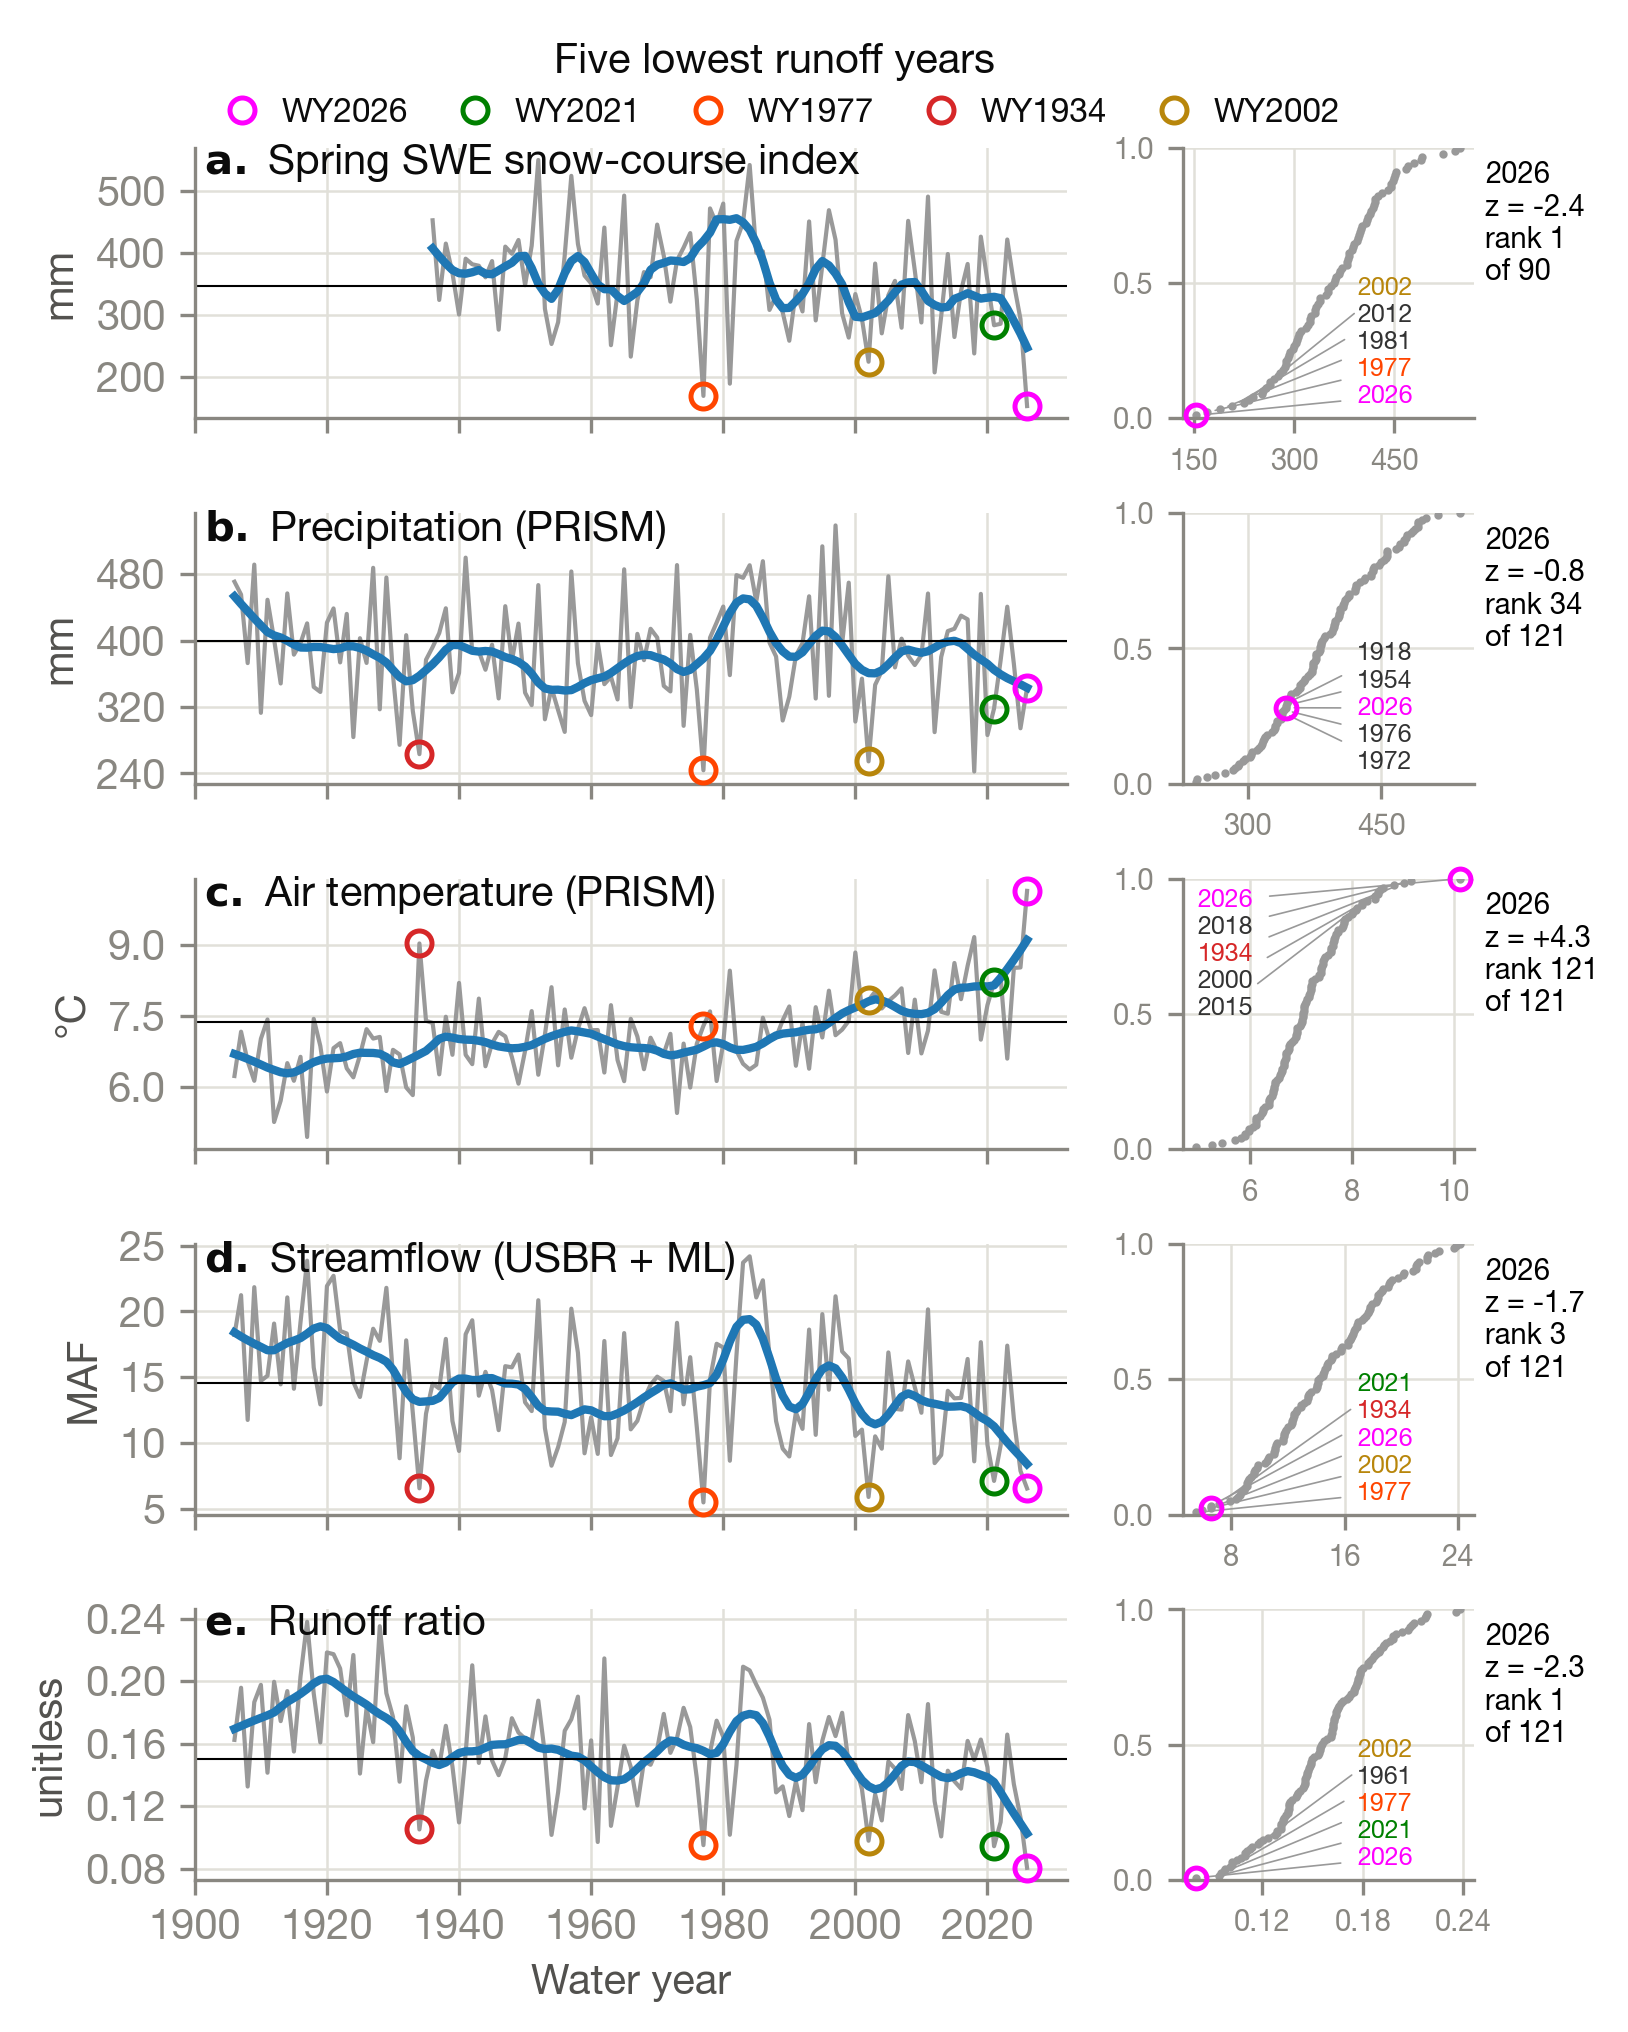
\includegraphics[]{figures/basic_flow_p_t_eff.png}\label{fig:historical}
    \caption{\textbf{How anomalous was WY2026?} Left: A timeseries of SWE, precipitation, temperature, streamflow, and runoff ratio (the ratio of total runoff to precipitation) for the Upper Colorado River at Lee's Ferry from 1904 to present. Snow surveys started in 1936. These data are all direct observations or based on observations. Right: the same, but the CDF of each variable. 2026 is highlighted in magenta and the four most similar years for each variable are displayed in text. The rank and z-score of 2026 is also displayed as text.}
\end{figure}



\begin{figure}
    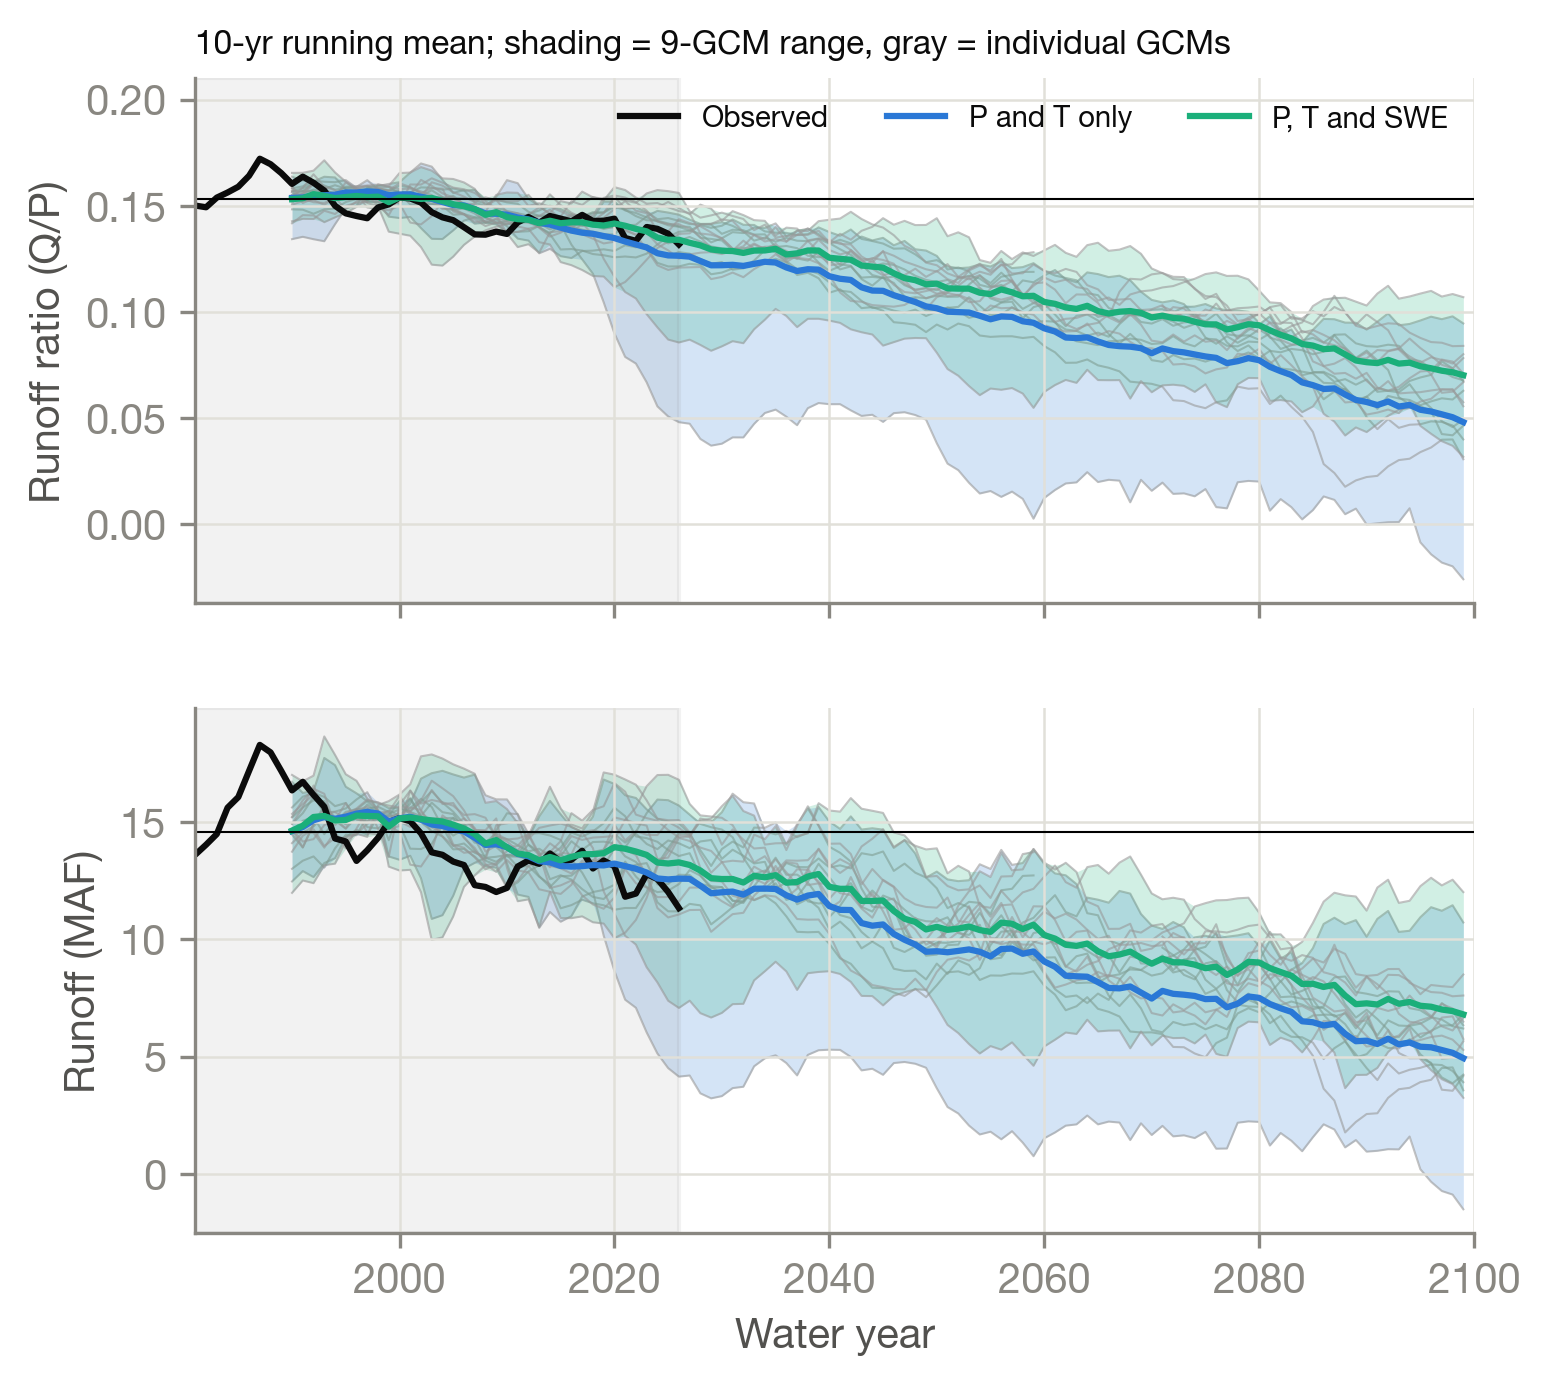
\includegraphics[]{figures/projected_q_wusd3.png}
    \caption{Projected changes in Runoff ratio (top) and Runoff (in million acre feet) under the SSP3-7.0 for 9 GCMs downscaled and bias-corrected by WUS-D3 (Table \ref{tab:gcms}). 
    Projections use WUS-D3 model P and T and the observationally constrained model of runoff sensitivity. 
    }
\end{figure}

\clearpage 

\section{Appendix}
\section{Methods}
We start from the decomposition framework used in several studies \cite{Lehner2019-hs,Milly2020-nk} (more),
extended to include snow. We let
\begin{equation}
\Delta Q = \alpha \Delta P + \beta \Delta T + \epsilon_q ,
\label{eq:q_model}
\end{equation}
where $\Delta X = (X - \bar{X})/\bar{X}$ for runoff, precipitation and SWE, $\Delta T = T - \bar{T}$,
and the bar denotes the WY1981--2010 mean. All regressions are fit without an intercept.

Spring snow water storage (SWE) may exert an independent effect on runoff, but it is itself
strongly correlated with precipitation and air temperature. We model the spring SWE anomaly similarly,
\begin{equation}
\Delta SWE = s_p \Delta P + s_t \Delta T + \epsilon_s ,
\label{eq:swe_model}
\end{equation}
where $\epsilon_s$ is the part of the SWE anomaly not explained by $\Delta P$ and $\Delta T$.
Substituting Eq.~\ref{eq:swe_model} into Eq.~\ref{eq:q_model} gives
\begin{equation}
\Delta Q = (\alpha + \gamma s_p)\, \Delta P + (\beta + \gamma s_t)\, \Delta T + \gamma \epsilon_s + \epsilon_q .
\label{eq:q_total}
\end{equation}
In Eq.~\ref{eq:q_model}, $\alpha$ and $\beta$ are the direct effects of precipitation and
temperature with SWE held fixed. The coefficients in Eq.~\ref{eq:q_total},
$\alpha + \gamma s_p$ and $\beta + \gamma s_t$, are the total effects ($\alpha_{tot}$, $\beta_{tot}$), including the part
that acts through snow. 
These total effects should correspond to the precipitation elasticity and
temperature sensitivity reported by \citeA{Lehner2019-hs} and \citeA{Milly2020-nk}. 


\section{Previous literature}

\begin{itemize}
\item \citeA{Woodhouse2016-tb} "In most recent drought years, low flows have been further exacerbated by warm temperatures". "Our work suggests warming temperatures are playing an increasingly important role in causing runoff declines even in nondrought years". \textcolor{blue}{They do not look at SWE, just precipitation, temperature, and soil moisture}.

\item \citeA{Nowak2012-qr}. Looks at runoff efficiency explicitly. "Per degree warming, a 14\% decrease in UCRB discharge was implied by the diagnosis of historical Lees Ferry streamflow and climate data." \textcolor{blue}{This might be the first study to show that temperature matters for runoff ratio in the UCRB}

\item \citeA{Lehner2017-se} "Because the recent decades have also been marked by substantial upward temperature trends, the question of whether runoff ratio declines can be linked to temperature increases, and thus potentially to anthropogenic global warming, has gained the attention of the water management community". 
"... we estimate that in years with below-median precipitation, very low (<10th percentile) runoff ratios are 2.5–3 times more likely if temperatures are warmer than normal (above-median)."

\item \citeA{Nolin2026-dc} 

\item \citeA{Palumbo2025-ru} 


\end{itemize}

\section{Data and Methods}

\begin{itemize}
\item \textbf{Runoff}: Lee's ferry naturalized streamflow  (\url{https://www.usbr.gov/lc/region/g4000/NaturalFlow/provisional.html}). 
\item \textbf{Precipitation and temperature}: PRISM Long-term 1895-present (get citation). Monthly and annual precipitation total in the UCRB.
\item \textbf{temperature}: NOAA USHCN monthly (station) data. This is a more homogenized dataset than PRISM. These are single stations only, but, we can compare the anomaly to the PRISM air temperature anomaly. They are very similar. This bolsters the point that PRISM data is fit for purpose.
\item \textbf{Peak SWE}: 1936 to present. I downloaded data from NRCS ``COOP" snow course surveys. The data are downloaded from \url{https://wcc.sc.egov.usda.gov/awdbRestApi/swagger-ui/index.html}. There are 16 snow courses that have springtime survey data between 1936 to present.
\item \textbf{Projections of temp, precipitation, and SWE}: WUS-D3. I'm using the bias-corrected version of \cite{Rahimi2024-gl} for 9 different GCMs under the SSP3-7.0 scenario with data from 1980 - end of century.
\end{itemize}


\begin{table}
\caption{CMIP6 GCMs dynamically downscaled in WUS-D3 \cite{Rahimi2024-gl} and used to drive the runoff ratio projections. FGOALS-g3 is excluded because of an artifact in its September precipitation.}
\centering
\begin{tabular}{l l l l}
\hline
GCM & Variant  \\
\hline
ACCESS-CM2    & r5i1p1f1  \\
CanESM5       & r1i1p2f1  \\
CESM2         & r11i1p1f1 \\
CNRM-ESM2-1   & r1i1p1f2  \\
EC-Earth3-Veg & r1i1p1f1  \\
EC-Earth3     & r1i1p1f1  \\
GISS-E2-1-G   & r1i1p1f2  \\
MIROC6        & r1i1p1f1  \\
MPI-ESM1-2-LR & r7i1p1f1  \\
\hline
\end{tabular}
\label{tab:gcms}
\end{table}




\bibliography{references}

\end{document}
